\chapter{Ottimizzazione}
L’High Performance Computing richiede, come suggerisce il nome stesso, di ottenere la massima efficacia dal codice sulla macchina su cui viene eseguito. L’ottimizzazione in HPC non è un’operazione singola, ma un bilanciamento di diversi vincoli: tempo di esecuzione, uso della memoria, efficienza energetica, robustezza e costi di I/O.
\section{Misurazione delle performance}
Quando parliamo di performance cerchiamo di andare a fare una stima di quanto il nostro codice riesca a sfruttare delle specifiche risorse della CPU. In particolare, ci concentriamo su:
\begin{itemize}
    \item Quanto è \textbf{veloce} il nostro codice.
    \item Quanto bene sfrutta il parallelismo a livello di istruzione.
\end{itemize}
\subsection{Misure sul clock}
Per quanto riguarda la velocità, sappiamo che la CPU non lavora in maniera continua ma lavora seguento \textbf{cicli di clock} il cui ritmo è di parecchi clock al secondo. La frequenza può anche variare a seconda del carico di lavoro aumentando o diminuendo per risparmiare energia. Nello specifico, ci riferiremo a questo fenomeno come \textbf{throttling}.

Proprio perché il ciclo di clock varia, misurare semplicemente il tempo di esecuzione potrebbe portare a stime imprecise. Può essere più comodo andare a vedere \textbf{quanti cicli di clock sono stati spesi} su una certa sezione di codice. In particolare, ci concentriamo su sezioni di codice che ripetono blocchi d'istruzioni su un array che rappresentano i punti più pesanti computazionalmente del nostro software. Questa metrica prende il nome di \textbf{Cyles Per Elemment} o \textbf{CPE}. Se vogliamo, il CPE rappresenta il numero di cicli di clock necessari all'analisi di una singola porzione di dato come, ad esempio, un singolo elemento dell'array. 

Al contrario, nel caso volessimo stimare quanto bene stiamo sfruttando la capacità super-scalare della CPU, ha più senso usare la metrice di \textbf{Istruzioni per Ciclo (IPC)} per valutare quante istruzioni per ciclo vengono eseguite. Questo ci darà l'informazione riguardo a quante operazioni stiamo riuscendo a fare contemporaneamente all'interno di un ciclo di clock.
\subsection{Misure sul Tempo}
Nonostante le misure sul clock siano sicuramente molto utili e precise, spesso si preferisce andare a ragionare in termini di \textbf{Tempo di esecuzione}. Fondamentalmente, guarderemo tre diversi tipi di tempo:
\begin{itemize}
    \item \textbf{Wall-clock time}: Fondamentalmente questo è il tempo d'orologio dall'inizio alla fine del processo. 
    \item \textbf{System-Time}: quantità di tempo che l'intero sistema trascorre eseguendo il codice. Questo comprende il tempo in \textbf{kernel mode}.
    \item \textbf{Process user-Time}: Metrica che tiene il tempo speso dalla CPU per eseguire le istruzioni del codice eliminando, in pratica, i tempi morti d'attesa. Questo è il tempo in \textbf{user mode}
    \item \textbf{CPU time}: Somma di system time e process user time.
\end{itemize}
Indipendentemente dalle metriche che stiamo accumulando, affrontare solo una misura non è una buona stima: bisogna fare la media su molte esecuzioni e sottrarre l’overhead della funzione di tempo stessa. 

Per misurare questi tempi in C possiamo utilizzare principalmente funzioni come \textit{gettimoofday()} che restituisce il wall clock time, \textit{clock()} che restituisce la somma tra lo user time e il system time e, infine, \textit{clock\_gettime()} che ritorna vari tipi di tempi tra cui real time, monotonic ecc. 
\begin{figure}[H]
    \centering
    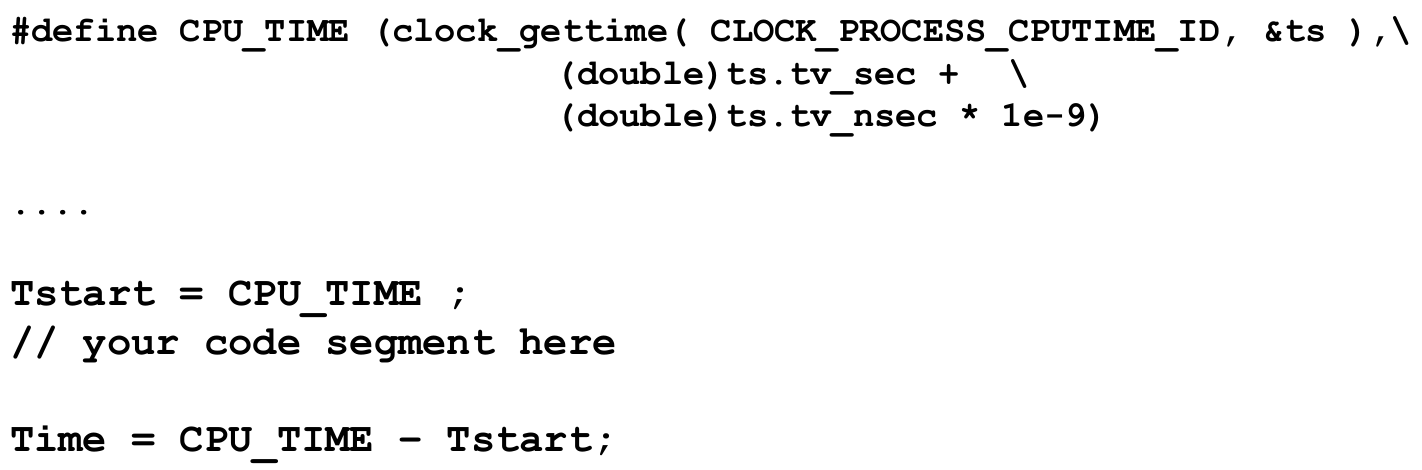
\includegraphics[width=0.75\linewidth]{Images/cap_3/clock_time.png}
\end{figure}
Come si vede in figura, è possibile misurare il tempo effettuato in una sezione di codice incapsulandolo tra i due CPU time. 

Un'altra cosa da tenere in considerazione è che il nostro processore, al giorno d'oggi, è \textbf{multi-core} e, spesso, i processi possono spostarsi tra un core e l'altro. Di fatto ciò comporta dei rallentamenti a causa del fatto che è necessario nuovamente riprendere i dati in memoria e metterli nella cache allocata per ogni singolo core (vedremo dopo in dettaglio). Per evitare questo, si usano delle funzioni particolare che effettuano un binding di un processo ad uno o più core.
\subsection{Profiling}
Il \textbf{profiling} è una fase cruciale del \textit{Performance Engineering}. Consiste nell'analizzare l'esecuzione di un programma utilizzando carichi di lavoro (\textit{workload}) reali per identificare i \textbf{punti critici} (\textit{hotspots}) e i \textbf{colli di bottiglia} del codice. 

Invece di procedere per tentativi, il profiling permette di guidare il processo di ottimizzazione basandosi su dati oggettivi. Un'analisi accurata permette di individuare:

\begin{itemize}
    \item \textbf{Intensità di calcolo e dati:} identifica quali specifiche linee di codice eseguono il maggior numero di operazioni o richiedono lo spostamento di grandi volumi di dati.
    \item \textbf{Stalli delle risorse:} rileva i punti in cui la CPU è ferma in attesa (ad esempio a causa di \textit{pipeline stalls} o latenze della memoria).
    \item \textbf{Efficienza dell'I/O:} traccia il tempo speso nelle operazioni di input/output, evidenziando schemi di accesso al disco inefficienti.
    \item \textbf{Bilanciamento del carico (Workload balance):} fondamentale in ambito parallelo, serve a capire se il lavoro è distribuito equamente tra i core o se ci sono processi che rallentano l'intera esecuzione.
\end{itemize}
Questa pratica la vedremo dopo nel dettaglio.

\section{Ottimizzare}
Come abbiamo detto, ottimizzare vuol dire \textbf{estrarre la massima efficacia del codice sulla macchina su cui viene eseguito}. È importante notare come sottolineiamo il fatto che questo processo sia riferito a una specifica macchina questo perché, a causa di dimensioni di memoria e simili, alcune scelte prese potrebbero essere ottimali su una macchina ma non sull'altra.

Inoltre, è necessario definire su cosa vogliamo ottimizzare. Questo perché potrebbe non essere possibile ottimizzare un codice a tutto tondo, ma potrebbe essere necessario dover trovare compromessi. Tra le varie condizioni di cui tener conto quando vogliamo ottimizzare, troviamo:
\begin{itemize}
    \item Vincoli di tempo;
    \item Vincoli di memoria;
    \item Vincoli di I/O;
    \item Desiderio di robustezza del sistema;
    \item Limiti energetici.
\end{itemize} 

Per quanto adesso il nostro focus sia incentrato sull'ottimizzazione del codice, è bene ricordare che prima di tutto dobbiamo:
\begin{itemize}
    \item Verificare la \textbf{correttezza} del codice. Cioè che faccia già correttamente quello che deve fare.
    \item Usare il giusto \textbf{modello di dati} in termini di struttura dati ecc.
    \item Scegliere il giusto \textbf{algoritmo}.
    \item Avere un \textbf{buon codice} che sia chiaro, pulito, conciso e documentato. Un codice sporco è difficile da ottimizzare perché nasconde le inefficienza. Usare il principio \textbf{DRY (Don’t Repeat Yourself)} evita il debito tecnico e facilita il debug. Inoltre, è bene che il codice sia \textbf{commentato}.
    \item Un'altra cosa da tenere in considerazione è il \textbf{Design} che comprende, in genere:
        \begin{itemize}
            \item Teoria, quindi lettura di come si svolgono solitamente le cose.
            \item Analisi dei vincoli e delle risorse che si hanno a disposizione.
            \item Traduzione della teoria in codice computabile.
            \item Testing che consiste nel verificare che tutto il codice o specifiche sezioni funzionino come ci si aspetta.
            \item Validazione per assicurarci che il codice faccia ciò che deve fare e verificare per assicurarci che il codice faccia ciò che fa correttamente.
        \end{itemize}
\end{itemize}
Un codice meravigliosamente ottimizzato che adotta l'algoritmo sbagliato è un controsenso, perché un algoritmo migliore, anche se implementato male, batterà (quasi) sempre il codice precedente per un numero di casi sufficientemente ampio.

In sintesi dovremmo lavorare come segue:
\begin{enumerate}
    \item Scrivere un programma che ci dia le risposte corrette e che si comporti correttamente sempre.
    \item Adottare gli algoritmi e le strutture dati più adatti ai nostri vincoli.
    \item Avere un codice sorgente pulito e ottimizzabile dal compilatore.
    \item Ottenere un flusso di lavoro basato sui dati e sui compiti.
    \item Verificare il codice in diverse condizioni anche non direttamente dipendenti dal codice stesso come i vari carichi di lavoro ecc. per trovare i colli di bottiglia e le inefficienze.
    \item Applicare tecniche di ottimizzazioni modificando i punti critici nel codice per rimuovere i blocchi di ottimizzazione.
    \item Tornare a 1 se necessario.
\end{enumerate}
Il \textbf{compilatore} è un programma che traduce il linguaggio sorgente in un linguaggio target equivalente
Un \textbf{interprete} è un programma di elaborazione del linguaggio che esegue direttamente un programma in un \textbf{linguaggio sorgente}.
La compilazione fa parte di una \textbf{pipeline} che traduce il codice sorgente in un codice eseguibile dalla macchina. Questa pipeline comprende:
\begin{itemize}
    \item \textbf{Preprocessore}: Analizza il sorgente includendo gli header ed espandendo le macro.
    \item \textbf{Front-end}: Traduce il sorgente in un linguaggio ad alto livello di astrazione specifico. Spesso assemby.
    \item \textbf{Assembler}: Produce il codice macchina dall'assemby generato.
    \item \textbf{Linker}: Risolve i riferimenti e gli indirizzi di memoria tra diverse sezioni del codice e librerie esterne.
\end{itemize}
I compilatori sono anche in grado di eseguire un’analisi sofisticata del codice sorgente in modo da produrre un codice target (solitamente un codice assembly) altamente ottimizzato per una data architettura target. Quindi, per prima cosa, lasciamo fare il lavoro al compilatore. 
Esistono diversi livelli di ottimizzazione generati automaticamente dal compilatore mediante specifico flag \textbf{-On}:
\begin{itemize}
    \item \texttt{-O0}: Nessuna ottimizzazione (default), utile per il debug.
    \item \texttt{-O1, -O2, -O3}: Livelli crescenti di aggressività. \textbf{Nota bene}: non è detto che\texttt{-O3}, sebbene spesso generi un
    codice più veloce, sia ciò di cui hai realmente bisogno; su alcune architetture può generare codice troppo voluminoso che satura le cache, rendendo preferibile \texttt{-Os} (ottimizzazione per dimensione).
    \item \texttt{-march=native}: Istruisce il compilatore a generare codice specifico per l'architettura della CPU su cui sta girando, sfruttando tutti i set di istruzioni (ISA) disponibili. Infatti, il compilatore generalmente produce un codice portabile, cioè un codice che può essere eseguito su qualsiasi CPU appartenente a quella classe di architettura.
\end{itemize}
Esistono anche diversi modelli tipici di compilazione come, ad esempio \textbf{fbrach-probabilities} o \textbf{fprofile-generate}.

Altra cosa utile che approfondiremo maggiormente anche dopo è l'uso di \textbf{memoria contigua} che, in quanto contigua, evita continui salti da un punto di memoria a un altro.

Esistono anche diverse classi di storage:
\begin{itemize}
    \item extern: variabili globali che esistono per sempre.
    \item auto: variabili locali allocate sullo stack.
    \item register: variabili che suggeriamo al compilatore di tenere in registro perché magari molto usata.
\end{itemize}
Inoltre, esistono anche dei quantificatori di variabili:
\begin{itemize}
    \item \textbf{const}: indica che il valore dentro la variabile non cambia mai.
    \item \textbf{volatile}: indica che la variabile è modificabile dall'esterno del programma.
    \item \textbf{restrict}: indica che l'indirizzo di memoria è accessibile solo tramite specifico puntatore.
\end{itemize}
\subsection{Memory Aliasing}
Il \textbf{Memory Aliasing} si verifica quando due o più riferimenti (puntatori) puntano alla stessa posizione di memoria. Questo è uno dei maggiori blocchi alle prestazioni in C/C++.
\begin{figure}[H]
    \centering
    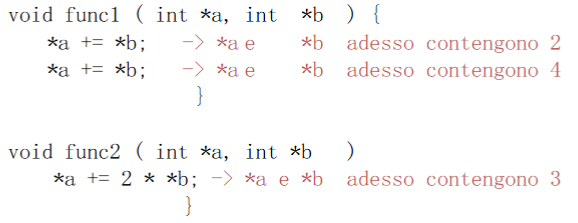
\includegraphics[width=0.75\linewidth]{Images/cap_3/aliasing.png}
\end{figure}
Consideriamo queste due funzioni. In effetti, se a e b puntano a due indirizzi diversi, il risultato delle due funzioni è lo stesso. Il discorso cambia, invece, quando a e b puntano allo stesso indirizzo come mostrato in figura.

Se il compilatore non può garantire che due puntatori siano distinti, non può ottimizzare gli accessi alla memoria perché teme che una scrittura su uno possa influenzare il valore dell'altro. Questo costringe la CPU a ricaricare continuamente i dati dalla memoria centrale anziché usare i registri o la cache. Per risolvere questo problema usiamo il qualificatore \textit{restrict}.

In generale è utile:
\begin{itemize}
    \item Scrivere codice evitando aliasing di memori rendendo chiaro a cosa serve una variabile e quando e mantenendo sotto controllo i branch condizionali.
    \item Usare strutture dati buone cache-friendly facendo sì che dati che vengono usati insieme, siano insieme. Inoltre, è necessario evitare il \textbf{false-sharing} che accade quando due thread lavorano su variabili diverse che però sfortunatamente risiedono nella stessa linea di cache, costringendo i core a invalidarsi la memoria a vicenda continuamente.
    \item Avere un buon flusso di lavoro così ché il compilatore possa ottimizzare i branch e gli accessi alla memoria.
    \item Sfruttare le architetture multi-core superscalari e out of order.
\end{itemize}